%% Reference https://docs.google.com/document/d/e/2PACX-1vTL8p8euifAho6K6PSE_b63A1HTucl3GCyLJSvjGq7ySnncqTnFa8azPNoMpzG9Wx38p4jPzxaC3OZg/pub#h.z11rqsgxo2dh

%%
%% Commands for TeXCount
%TC:macro \cite [option:text,text]
%TC:macro \citep [option:text,text]
%TC:macro \citet [option:text,text]
%TC:envir table 0 1
%TC:envir table* 0 1
%TC:envir tabular [ignore] word
%TC:envir displaymath 0 word
%TC:envir math 0 word
%TC:envir comment 0 0
%%
\documentclass[sigconf,11pt]{acmart}

\settopmatter{printacmref=false}
\renewcommand\footnotetextcopyrightpermission[1]{}

\usepackage{titlesec}
\titleformat*{\section}{\fontsize{14}{15}\selectfont}

%% \BibTeX command to typeset BibTeX logo in the docs
\AtBeginDocument{%
  \providecommand\BibTeX{{%
    \normalfont B\kern-0.5em{\scshape i\kern-0.25em b}\kern-0.8em\TeX}}}

%% Rights management information.  This information is sent to you
%% when you complete the rights form.  These commands have SAMPLE
%% values in them; it is your responsibility as an author to replace
%% the commands and values with those provided to you when you
%% complete the rights form.
% \setcopyright{none}
% \copyrightyear{}
% \acmYear{}
% \acmDOI{}

%% These commands are for a PROCEEDINGS abstract or paper.
% \acmConference[CSE6242]{Make sure to enter the correct
%   conference title from your rights confirmation emai}{Sept 01,
%   2022}{Atlanta, GA}
%
%  Uncomment \acmBooktitle if th title of the proceedings is different
%  from ``Proceedings of ...''!
%
%\acmBooktitle{Woodstock '18: ACM Symposium on Neural Gaze Detection,
%  June 03--05, 2018, Woodstock, NY}
% \acmPrice{}
% \acmISBN{}



%%
%% For managing citations, it is recommended to use bibliography
%% files in BibTeX format.
%%
%% You can then either use BibTeX with the ACM-Reference-Format style,
%% or BibLaTeX with the acmnumeric or acmauthoryear sytles, that include
%% support for advanced citation of software artefact from the
%% biblatex-software package, also separately available on CTAN.
%%
%% Look at the sample-*-biblatex.tex files for templates showcasing
%% the biblatex styles.
%%

%%
%% The majority of ACM publications use numbered citations and
%% references.  The command \citestyle{authoryear} switches to the
%% "author year" style.
%%
%% If you are preparing content for an event
%% sponsored by ACM SIGGRAPH, you must use the "author year" style of
%% citations and references.
%% Uncommenting
%% the next command will enable that style.
%%\citestyle{acmauthoryear}

%%
%% end of the preamble, start of the body of the document source.
\begin{document}

%%
%% The "title" command has an optional parameter,
%% allowing the author to define a "short title" to be used in page headers.
\title{\Large Analyzing the Implicit Social Network from GitHub Activities}

%%
%% The "author" command and its associated commands are used to define
%% the authors and their affiliations.
%% Of note is the shared affiliation of the first two authors, and the
%% "authornote" and "authornotemark" commands
%% used to denote shared contribution to the research.
\author{\normalsize Ran Tavory, Ruzvidzo Ngulube, Jonathan del Campo, Brendan Danyluik (Dropping)}

% Display extended author information if we want to

% \affiliation{%
%   \institution{Georgia Institute of Technology}
%   \city{Atlanta}
%   \state{GA}
%   \country{USA}
% }

% \authornote{Authors contributed equally to this research.}
% \email{trovato@corporation.com}
% \orcid{1234-5678-9012}
% \author{G.K.M. Tobin}
% \authornotemark[1]
% \email{webmaster@marysville-ohio.com}
% \affiliation{%
%   \institution{Institute for Clarity in Documentation}
%   \streetaddress{P.O. Box 1212}
%   \city{Dublin}
%   \state{Ohio}
%   \country{USA}
%   \postcode{43017-6221}
% }

% \author{Lars Th{\o}rv{\"a}ld}
% \affiliation{%
%   \institution{The Th{\o}rv{\"a}ld Group}
%   \streetaddress{1 Th{\o}rv{\"a}ld Circle}
%   \city{Hekla}
%   \country{Iceland}}
% \email{larst@affiliation.org}

% \author{Valerie B\'eranger}
% \affiliation{%
%   \institution{Inria Paris-Rocquencourt}
%   \city{Rocquencourt}
%   \country{France}
% }

% \author{Aparna Patel}
% \affiliation{%
%  \institution{Rajiv Gandhi University}
%  \streetaddress{Rono-Hills}
%  \city{Doimukh}
%  \state{Arunachal Pradesh}
%  \country{India}}

% \author{Huifen Chan}
% \affiliation{%
%   \institution{Tsinghua University}
%   \streetaddress{30 Shuangqing Rd}
%   \city{Haidian Qu}
%   \state{Beijing Shi}
%   \country{China}}

% \author{Charles Palmer}
% \affiliation{%
%   \institution{Palmer Research Laboratories}
%   \streetaddress{8600 Datapoint Drive}
%   \city{San Antonio}
%   \state{Texas}
%   \country{USA}
%   \postcode{78229}}
% \email{cpalmer@prl.com}

% \author{John Smith}
% \affiliation{%
%   \institution{The Th{\o}rv{\"a}ld Group}
%   \streetaddress{1 Th{\o}rv{\"a}ld Circle}
%   \city{Hekla}
%   \country{Iceland}}
% \email{jsmith@affiliation.org}

% \author{Julius P. Kumquat}
% \affiliation{%
%   \institution{The Kumquat Consortium}
%   \city{New York}
%   \country{USA}}
% \email{jpkumquat@consortium.net}

%%
%% By default, the full list of authors will be used in the page
%% headers. Often, this list is too long, and will overlap
%% other information printed in the page headers. This command allows
%% the author to define a more concise list
%% of authors' names for this purpose.
% \renewcommand{\shortauthors}{Trovato and Tobin, et al.}

\begin{abstract}
  We develop a method of mining GitHub event activity to construct an implicit social network
  between GitHub users encompassing their GitHub repositories and the connections between them.
  We then utilize this network for interesting visualizations, including shortest path between users
  and finding the most influential users.
\end{abstract}


%%
%% Keywords. The author(s) should pick words that accurately describe
%% the work being presented. Separate the keywords with commas.
% \keywords{GitHub, Social Network, Visualization}

%% A "teaser" image appears between the author and affiliation
%% information and the body of the document, and typically spans the
%% page.
% \begin{teaserfigure}
%   \includegraphics[width=\textwidth]{fig/sampleteaser.pdf}
%   \caption{Seattle Mariners at Spring Training, 2010.}
%   \Description{Enjoying the baseball game from the third-base
%   seats. Ichiro Suzuki preparing to bat.}
%   \label{fig:teaser}
% \end{teaserfigure}

%%
%% This command processes the author and affiliation and title
%% information and builds the first part of the formatted document.
\maketitle
\pagestyle{plain}

\section*{What are you trying to do?}
Create an interactive UI with a graph that allows querying the activity of GitHub users
and relations between GitHub users, in particular, find the shortest path between two users
(edges are defined by co-activity on the same project),
Similar to the Erdős number in Mathematics \cite{wiki:erdos}, rate users in terms of their
distance from some of GitHub "celebrity" user, for example distance from Linus Torvalds
and find the most influential users for a certain technology scope, e.g. D3.

Extracting implicit social graph structure has been suggested before,
for example \citeauthor{coding-together} \cite{coding-together} created a followers and contributors graphs
to calculate statistical measures such as the rich club coefficient \cite{wiki:rich-club-coefficient}.
\citeauthor{network-structure-social-coding}\cite{network-structure-social-coding} took a similar approach
of mining GitHub's event history to build a graph and compute statistics for this graph, such as
graph's connectivity, average shortest path and PageRank\cite{pagerank}

Identifying influential users or opinion leaders has its roots in sociology and in recent years has been
implemented in different internet systems using, one interesting comparison
between some of the methods is the focus of \citeauthor{identifying-top-n} in \cite{identifying-top-n}
where China's social network "Sina" and a local cluster of 4k students in Shanghai University are used
to compare the accuracy of three different opinion leaders discovery methods,
PageRank, HITS\cite{hits} and Synthesized Centrality (invented by the authors).
% The authors find that SC results in similar recall to PR and HITS but has higher precision.
% This is interesting to our work although the computational costs of SC is higher from other methods and we
% suspect that at our scale this may present challenges.

\citeauthor{influence-analysis-of-github-repositories}\cite{influence-analysis-of-github-repositories}
Through the usage of HITS analyzed graphs that show the influence and relationship between GitHub
repositories and users.
They studied how specific repositories influence the development of the code of other repositories,
and study how repositories rank over time.

From a slightly different angle \citeauthor{collaboration-strength-metrics-github}\cite{collaboration-strength-metrics-github}
studied the correlation between the properties that measure the strength of software social coding
collaboration on GitHub; Several ways to measure collaboration were presented, for example,
the Preferential Attachment (PA) which assumes that the more edges a node has (a user or a project),
the more likely it will get more edges.

\citeauthor{user-influence-analysis-github}\cite{user-influence-analysis-github} focused on a very specific
workflow of GitHub, namely the Follow-Star-Fork workflow and constructed a graph based on these activities.
They implemented several quantitative measures, specifically UserRank (like PageRank), HITS, H-index\cite{wiki:h-index},
Betweenness centrality\cite{betweenness}, Spearman rank correlation\cite{wiki:spearman},
and Borda Count voting\cite{wiki:borda} to measure the influence of a user.

\citeauthor{measuring-user-influence-github}\cite{measuring-user-influence-github} measured the influence
of GitHub users and specifically defined and quantified what does influence mean in GitHub and whether the measured
influence remains siloed to specific domain of content (e.g. technology or programming language).

\citeauthor{influence-github-stackoverflow}\cite{influence-github-stackoverflow} combined two software development
focused websites, GitHub and StackOverflow, to study the influence and contribution across these two networks.
After studying the characteristics of each separate network a combination of the networks is studied
as the correlation between the same user's activity in one network to the other.

% \citeauthor{identifying-influences-in-the-internet-era}\cite{identifying-influences-in-the-internet-era} researched
% Twitter to conduct Social Network Analysis (SNA) and identify Social Media Influencers (SMIs).
% They revealed the existence of three different SMI typologies: disseminator, engager and leader.
% Even though this study is conducted on Twitter, perhaps some of its methodology can be applied to GitHub.

\section*{Today's status and limitations}
We have not seen such interactive interface for GH as of today.
What we have seen is statistical analysis of GitHub's graph data (\cite{coding-together},
\cite{influence-analysis-of-github-repositories} and \cite{collaboration-strength-metrics-github})
but none of the resources we have surveyed allows for interactive discovery.

There are databases with raw GitHub data (\cite{ghtorrent}, \cite{gharchive} and \cite{bq-gh})
and there is an API for GitHub's data\cite{gh-api} but again, a tool that structures this data
in a social network structure to allow interactive discovery we did not find.

We plan to create an interactive interface such as the one studied by \citeauthor{do-you-know-the-way-to-sna}\cite{do-you-know-the-way-to-sna}
where a user usability study of the network analysis tool NodeXL is conducted and a set of guidelines of do's an don'ts is presented.
We do not intend to use NodeXL specifically, yet user study conclusions are useful.

\section*{Novelty in your approach and why will it be successful}
It is a simple way to discover connection between software developers and perhaps discover software developer communities.
This can be useful for businesses trying to reach out to certain communities and looking for thought leaders in those communities.
It can also be useful to any GitHub user trying to assess her contributions within GitHubs' community.

\section*{Who cares?}
Businesses may care about community discovery for marketing purposes.
Individuals may care about personal branding and achievements.

\section*{What impact will it make, and how to measure it?}
The project, if successful, would become a popular tool within developers and businesses
looking to study the social graph implied by GitHub, in particular finding connections to other specific users
and identifying communities and their thought leaders.

It has been claimed by \citeauthor{developer-onboarding-github}\cite{developer-onboarding-github}
that there is evidence for socialization as a precursor to joining a project
and so we believe that presenting the social graph would open doors to more cooperation between users.

A way to measure is by posting references to this project on reddit, twitter, hackernews and measure their
popularity and engagement.

\section*{What are the risks and payoffs?}
There are several notable risks, in particular - data may be difficult to obtain at scale.
Although there are multiple sources, from our research we know that no single source encompasses all the aspects
we require so we will have to merge multiple sources.
Merging successfully is risky as well as obtaining a complete view of the data at scale.
We've seen reports of missing data, incorrect data, inconsistent data and obfuscated data (for privacy reasons)\cite{promises-and-perils-mining-github}.

Data is large so there are scalability concerns including collection, preprocessing and serving.
How to properly handle such large data and provide fast enough access for an interactive user experience may be challenging.

Payoffs: first, community engagement. Later - perhaps a business opportunity.

\section*{How much will it cost?}
We will collect the data, process it (possibly on Spark) and
store it for serving in a graph database (Neo4j\cite{neo4j}).
Serving costs include the collector process (1 servers), a spark cluster (4 nodes or more),
one Node4j server and a web server.
Not counting networking and storage costs.
Back of the envelope calculation, assume each server costs 40cent per hour (EC2 \emph{m5.2xlarge})
and assume that for ongoing serving two servers are needed (Neo4j and Web) for 2 months (60 days)
and for the collection we need 4 servers (for the collection period, let's say 1 month),
we roughly have $\$0.4 \times 24 \times (2 \times 60 + 4 \times 30) = \$2304$.
This is not cheap and we will look for ways to get funding and reduce costs.

A cheaper alternative is by not using Spark and instead use a single server for everything,
processing, Neo4J and serving, this will cost between \$300-600 for 60 days, depending on hardware.

\section*{How long will it take?}
Data collection and processing can complete within one month and writing the interface on top of it will take another month
but these can be parallelized.

Table~\ref{tab:pow} summarizes the plan of work
% TODO: If we have more space ad items here
\begin{table}
  \caption{Plan of Work in high level, all work will be evenly distributed}
  \label{tab:pow}
  \begin{tabular}{cccl}
    \toprule
    Work item               & Who                         & Start   &  Duration\\
    \midrule
    Proposal document       & Ran               & Oct 8   & 3 days \\
    Proposal presentation   & Jonathan          & Oct 10  & 2 days \\
    Proposal video          & Ruzvidzo          & Oct 10  & 2 days \\
    Data Collection         & Jonathan and All  & Nov 1   & 4 weeks \\
    Data Augmentation       & Ruzvidzo          & Nov 7   & 3 weeks \\
    Web and UI              & Ran               & Nov 1   & 4 weeks\\
    Progress report         & All               & TBD     & 1 week \\
    Final report            & All               & TBD     & 2 weeks \\
  \bottomrule
\end{tabular}
\end{table}

% If we have more time then another interesting aspect of the data we process is a
% Sentiment Analysis of Developers' Comments on GitHub, as suggested by \citeauthor{sentiment-analysis}\cite{sentiment-analysis}.
% We could enhance our network analysis with an aggregation of the sentiment of the comments.

\section*{Final checks and progress measurement}
The riskiest part is data collection and processing so we plan to handle it first and all team will work on that.
Next up is the interactive UI.
And finally and internal usability study and testing.


% \section{Template Overview}
% As noted in the introduction, the ``\verb|acmart|'' document class can
% be used to prepare many different kinds of documentation --- a
% double-blind initial submission of a full-length technical paper, a
% two-page SIGGRAPH Emerging Technologies abstract, a ``camera-ready''
% journal article, a SIGCHI Extended Abstract, and more --- all by
% selecting the appropriate {\itshape template style} and {\itshape
%   template parameters}.

% URL
% \url{https://www.acm.org/publications/proceedings-template}.

% The primary parameter given to the ``\verb|acmart|'' document class is
% \begin{verbatim}
%   \documentclass[STYLE]{acmart}
% \end{verbatim}

% \begin{itemize}
% \item {\verb|acmsmall|}: The default journal template style.
% \item {\verb|acmlarge|}: Used by JOCCH and TAP.
% \item {\verb|acmtog|}: Used by TOG.
% \end{itemize}

% Bolding
% {\bfseries Your document will be returned to you for revision if
%   modifications are discovered.}


% \section{Tables}

% The ``\verb|acmart|'' document class includes the ``\verb|booktabs|''
% package --- \url{https://ctan.org/pkg/booktabs} --- for preparing
% high-quality tables.

% Table captions are placed {\itshape above} the table.

% Because tables cannot be split across pages, the best placement for
% them is typically the top of the page nearest their initial cite.  To
% ensure this proper ``floating'' placement of tables, use the
% environment \textbf{table} to enclose the table's contents and the
% table caption.  The contents of the table itself must go in the
% \textbf{tabular} environment, to be aligned properly in rows and
% columns, with the desired horizontal and vertical rules.  Again,
% detailed instructions on \textbf{tabular} material are found in the
% \textit{\LaTeX\ User's Guide}.

% Immediately following this sentence is the point at which
% Table~\ref{tab:freq} is included in the input file; compare the
% placement of the table here with the table in the printed output of
% this document.

% \begin{table}
%   \caption{Frequency of Special Characters}
%   \label{tab:freq}
%   \begin{tabular}{ccl}
%     \toprule
%     Non-English or Math&Frequency&Comments\\
%     \midrule
%     \O & 1 in 1,000& For Swedish names\\
%     $\pi$ & 1 in 5& Common in math\\
%     \$ & 4 in 5 & Used in business\\
%     $\Psi^2_1$ & 1 in 40,000& Unexplained usage\\
%   \bottomrule
% \end{tabular}
% \end{table}

% To set a wider table, which takes up the whole width of the page's
% live area, use the environment \textbf{table*} to enclose the table's
% contents and the table caption.  As with a single-column table, this
% wide table will ``float'' to a location deemed more
% desirable. Immediately following this sentence is the point at which
% Table~\ref{tab:commands} is included in the input file; again, it is
% instructive to compare the placement of the table here with the table
% in the printed output of this document.

% \begin{table*}
%   \caption{Some Typical Commands}
%   \label{tab:commands}
%   \begin{tabular}{ccl}
%     \toprule
%     Command &A Number & Comments\\
%     \midrule
%     \texttt{{\char'134}author} & 100& Author \\
%     \texttt{{\char'134}table}& 300 & For tables\\
%     \texttt{{\char'134}table*}& 400& For wider tables\\
%     \bottomrule
%   \end{tabular}
% \end{table*}

% Always use midrule to separate table header rows from data rows, and
% use it only for this purpose. This enables assistive technologies to
% recognise table headers and support their users in navigating tables
% more easily.

% \section{Math Equations}
% You may want to display math equations in three distinct styles:
% inline, numbered or non-numbered display.  Each of the three are
% discussed in the next sections.

% \subsection{Inline (In-text) Equations}
% A formula that appears in the running text is called an inline or
% in-text formula.  It is produced by the \textbf{math} environment,
% which can be invoked with the usual
% \texttt{{\char'134}begin\,\ldots{\char'134}end} construction or with
% the short form \texttt{\$\,\ldots\$}. You can use any of the symbols
% and structures, from $\alpha$ to $\omega$, available in
% \LaTeX~\cite{Lamport:LaTeX}; this section will simply show a few
% examples of in-text equations in context. Notice how this equation:
% \begin{math}
%   \lim_{n\rightarrow \infty}x=0
% \end{math},
% set here in in-line math style, looks slightly different when
% set in display style.  (See next section).

% \subsection{Display Equations}
% A numbered display equation---one set off by vertical space from the
% text and centered horizontally---is produced by the \textbf{equation}
% environment. An unnumbered display equation is produced by the
% \textbf{displaymath} environment.

% Again, in either environment, you can use any of the symbols and
% structures available in \LaTeX\@; this section will just give a couple
% of examples of display equations in context.  First, consider the
% equation, shown as an inline equation above:
% \begin{equation}
%   \lim_{n\rightarrow \infty}x=0
% \end{equation}
% Notice how it is formatted somewhat differently in
% the \textbf{displaymath}
% environment.  Now, we'll enter an unnumbered equation:
% \begin{displaymath}
%   \sum_{i=0}^{\infty} x + 1
% \end{displaymath}
% and follow it with another numbered equation:
% \begin{equation}
%   \sum_{i=0}^{\infty}x_i=\int_{0}^{\pi+2} f
% \end{equation}
% just to demonstrate \LaTeX's able handling of numbering.

% \section{Figures}

% The ``\verb|figure|'' environment should be used for figures. One or
% more images can be placed within a figure. If your figure contains
% third-party material, you must clearly identify it as such, as shown
% in the example below.
% \begin{figure}[h]
%   \centering
%   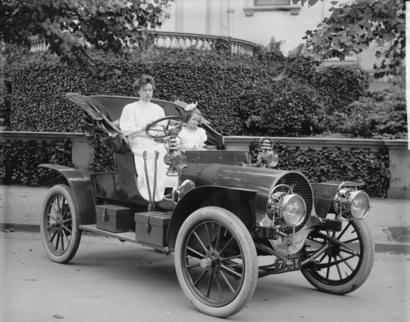
\includegraphics[width=\linewidth]{fig/sample-franklin.png}
%   \caption{1907 Franklin Model D roadster. Photograph by Harris \&
%     Ewing, Inc. [Public domain], via Wikimedia
%     Commons. (\url{https://goo.gl/VLCRBB}).}
%   \Description{A woman and a girl in white dresses sit in an open car.}
% \end{figure}

% Your figures should contain a caption which describes the figure to
% the reader.

% Figure captions are placed {\itshape below} the figure.

% Every figure should also have a figure description unless it is purely
% decorative. These descriptions convey what’s in the image to someone
% who cannot see it. They are also used by search engine crawlers for
% indexing images, and when images cannot be loaded.

% A figure description must be unformatted plain text less than 2000
% characters long (including spaces).  {\bfseries Figure descriptions
%   should not repeat the figure caption – their purpose is to capture
%   important information that is not already provided in the caption or
%   the main text of the paper.} For figures that convey important and
% complex new information, a short text description may not be
% adequate. More complex alternative descriptions can be placed in an
% appendix and referenced in a short figure description. For example,
% provide a data table capturing the information in a bar chart, or a
% structured list representing a graph.  For additional information
% regarding how best to write figure descriptions and why doing this is
% so important, please see
% \url{https://www.acm.org/publications/taps/describing-figures/}.

% \subsection{The ``Teaser Figure''}

% A ``teaser figure'' is an image, or set of images in one figure, that
% are placed after all author and affiliation information, and before
% the body of the article, spanning the page. If you wish to have such a
% figure in your article, place the command immediately before the
% \verb|\maketitle| command:
% \begin{verbatim}
%   \begin{teaserfigure}
%     \includegraphics[width=\textwidth]{sampleteaser}
%     \caption{figure caption}
%     \Description{figure description}
%   \end{teaserfigure}
% \end{verbatim}

%%
%% The next two lines define the bibliography style to be used, and
%% the bibliography file.

\pagebreak
\bibliographystyle{ACM-Reference-Format}
\bibliography{references}

\end{document}
\endinput
%%
%% End of file `sample-sigconf.tex'.
